%%%%%%%%%%%%%%%%%%%%%%%%%%%%%%%%%%%%%%%%%%%%
% 
% Last edits: Jan 4, 2017
%%%%%%%%%%%%%%%%%%%%%%%%%%%%%%%%%%%%%%%%%%%%

\documentclass[12pt]{article}
\usepackage{natbib}
\usepackage[letterpaper, margin=1.1in]{geometry}
\usepackage{graphicx}
\usepackage[table,xcdraw]{xcolor}
\usepackage{wrapfig}
\usepackage{enumitem}
\setlist[enumerate]{itemsep=0mm}
\usepackage{multirow}
\usepackage{lscape}
\usepackage{caption}
\usepackage{subcaption}
\usepackage{float}
\usepackage{hyperref}


\begin{document}
\noindent{Alexandra Pulwicki \\ \today}

\begin{center}
\Large \textbf{Methods\\ Data Processing}
\end{center}


\section*{Overview}
This section documents the process of going from raw data to processed and consolidated data that will be used for analysis in subsequent components of the project. A description of the various scripts used to process these data and the final data structure is outlined.


\tableofcontents
\pagebreak


%%%%
\section{Data processing}
%%%%

Converting snow depth and density measurements to usable values of snow water equivalent (SWE) is done using a number of scripts written in Matlab. Since there are a number of possible variations for how SWE is estimated, various options are outlined in the `OPTIONS.m' script. To run the entire data processing framework first ensure your desired SWE estimation options are reflected in the `OPTIONS.m' script and then run both `OPTIONS.m' and `MAIN.m'.

\subsection{Snow depth measured with graduated avalanche probe}

\subsubsection{Linear and curvilinear transect surveys}

\begin{wrapfigure}{R}{0.7\textwidth}
	\centering
	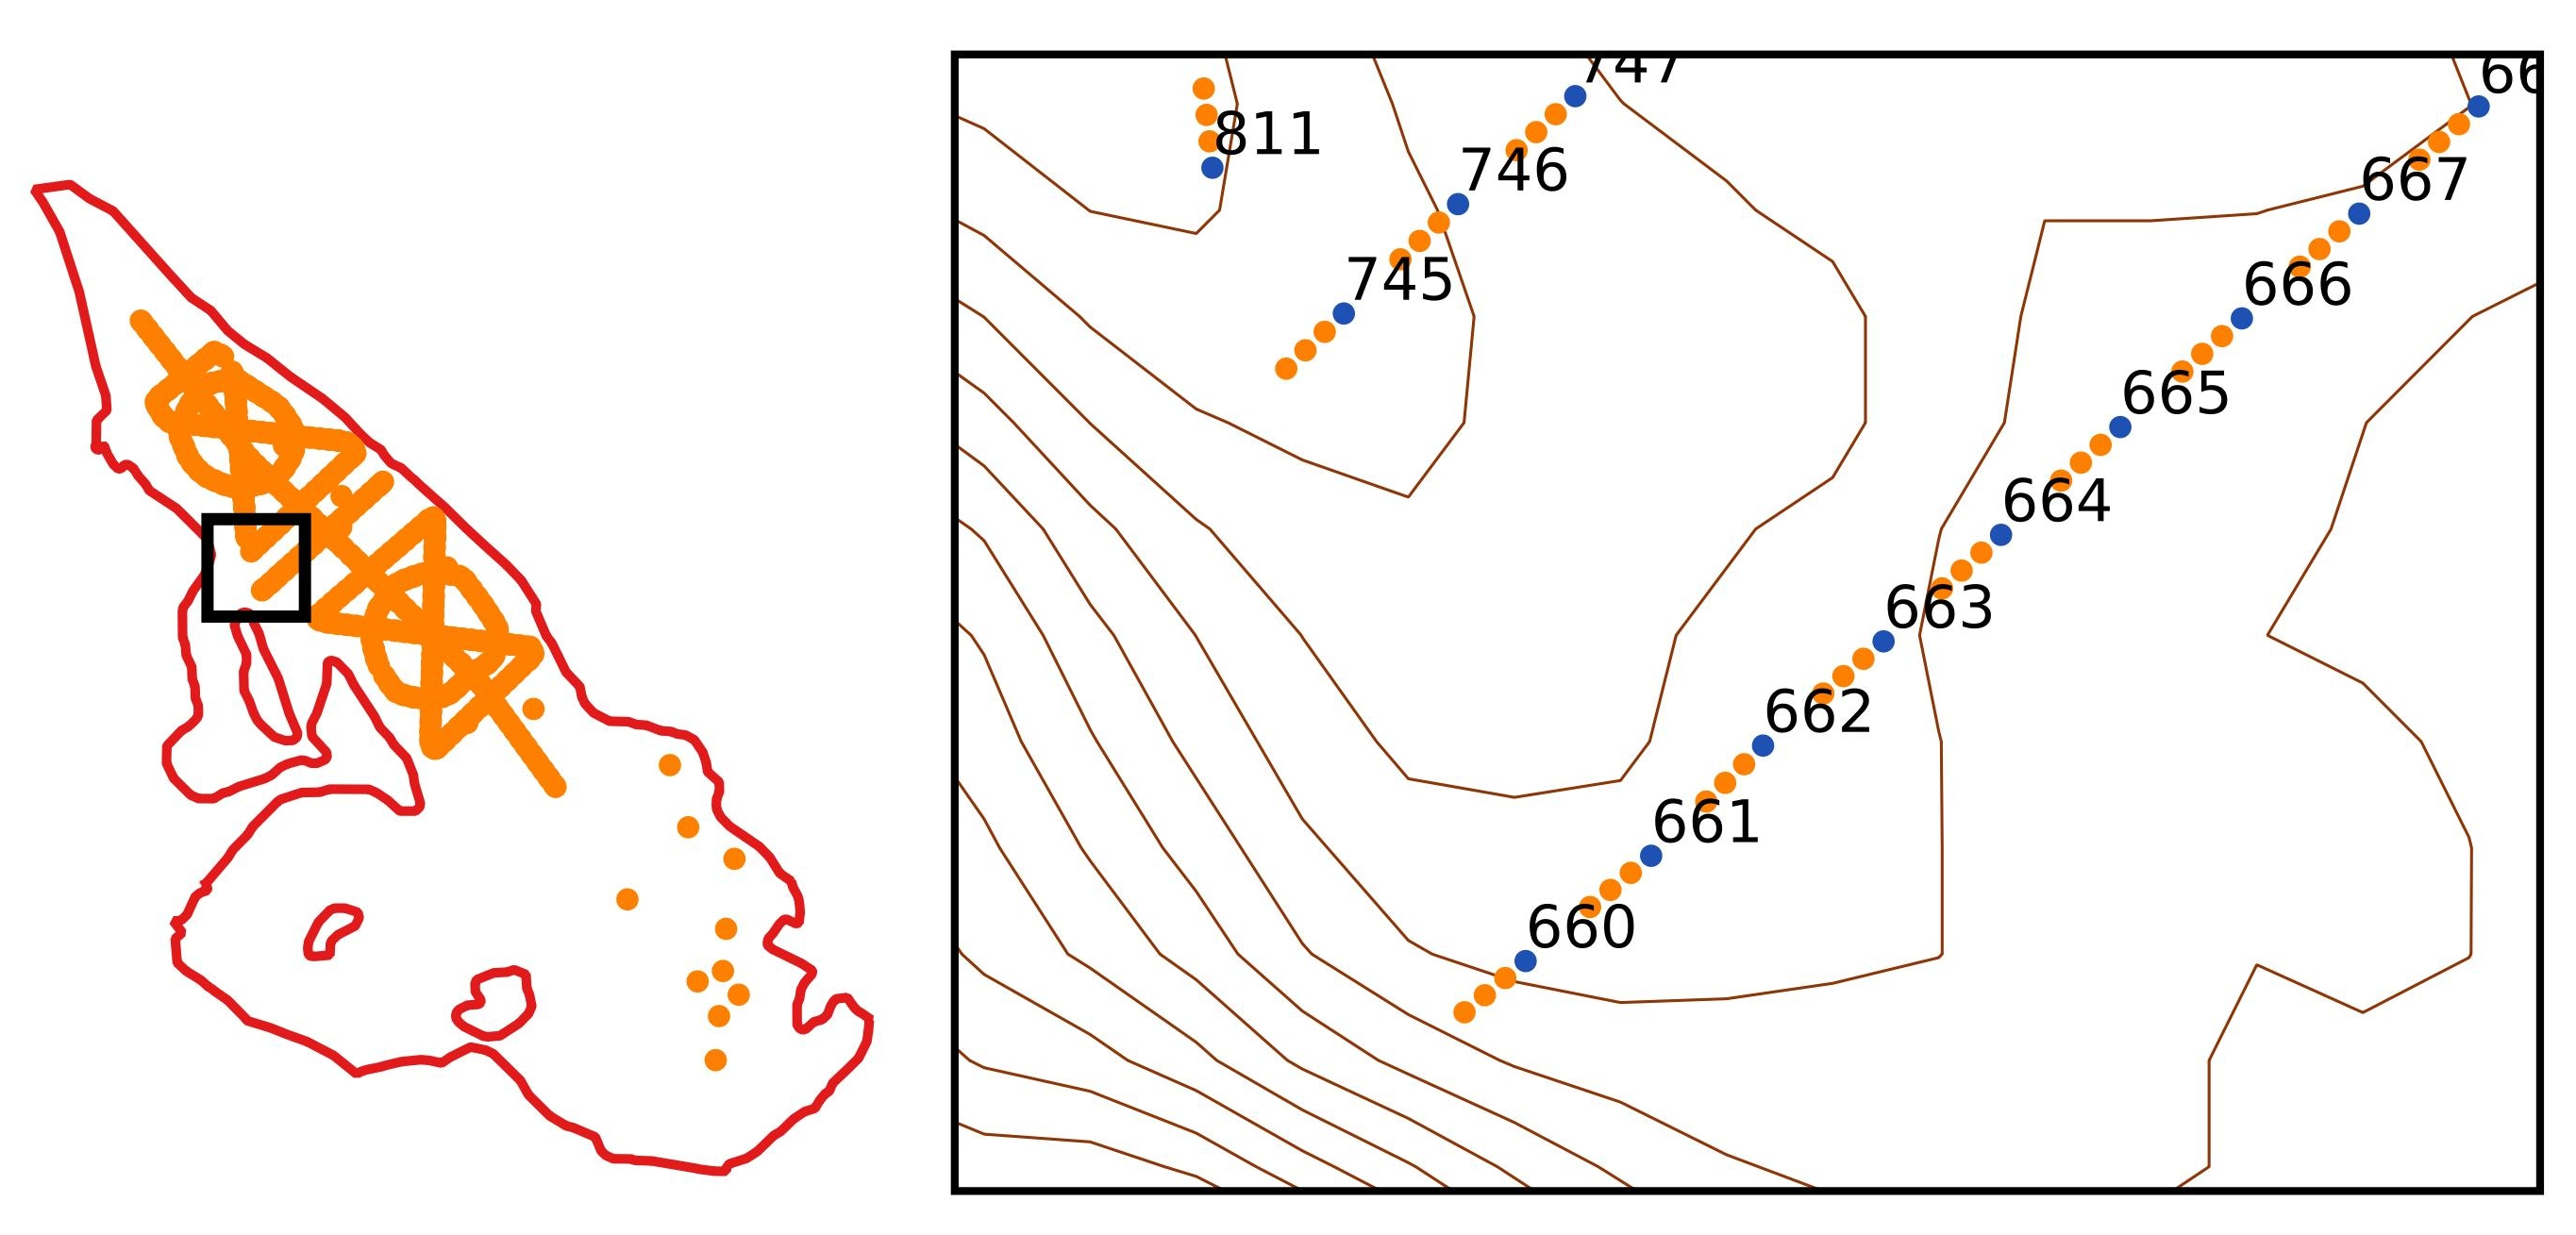
\includegraphics[width = 0.7\textwidth]{transect_measure_locations.jpeg}\\
	\caption{Example of estimating snow depth measurement locations in one area (indicted by black box) on Glacier 13. Numbered waypoint (WP) locations are shown in blue and estimated measurement locations are shown in orange at a distance of 10, 20, and 30 m from the WP. Measurement locations are taken to be along a straight line between subsequent WPs. For the first WP of a transect, the measurement locations are assumed to be along the same line as that between the first and second WPs of a transect. For example, the measurement locations behind WP 660 fall along the same line as those between WP 660 and WP 661. The same is true for WP 745. }
	\label{fig:transect_measure_loc}
\end{wrapfigure}

Snow depth measurements along the linear and curvilinear transects were taken at locations a certain distance from marked waypoints. Since only the coordinates of the waypoints (WP) were recorded, the measurement coordinates need to be estimated. The measurement locations were assumed to be 10, 20, and 30 m behind the marked WP, in a straight line between the marked WP and the previous WP (Figure \ref{fig:transect_measure_loc}). In cases with only two observers, locations were assumed to be 10 and 20 m behind the marked WP. For the first marked WP of a transect, it was assumed that the measurement locations were along the same line as that between the first and second WPs. The following methodology was used to determine measurement locations (each step corresponds with a section of the Matlab code `MeasurementLocations.m'): 
\begin{enumerate}
	\item Waypoint (WP) locations were exported from the GPS units using the Garmin BaseCamp program. They were then imported to QGIS and exported with UTM coordinates in the file `GlacierWP\_UTM.xlsx'. 
	\item In order to obtain the measurement locations for the first WPs of each pattern, a fictitious WP was created that was along the line between the first and second WPs, but located ahead of the first WP. These fictitious waypoints were then inserted into the original data. 
	\item A set of 1000 equally spaced points was created along a straight line between each set of subsequent of WPs (including the fictitious WPs from the previous step) using the function linspaceNDim.m created by Steeve Ambroise and downloaded from the MathWorks File Exchange. The Euclidean distance between these interpolated points and the marked WP was then calculated and the points with distances closest to the assumed separation between observers were retained. A matrix was then created, which has the UTM Zone 7N Easting and Northing of each measurement location and is labelled with the marked WP and a decimal that corresponds to the relative observer (e.g. label 45.2 means that the location was determined from the marked WP \#45 and is 20 m behind this WP because it is the second observer). 
\end{enumerate}

Data recorded by each observer in the field books were entered into a spreadsheet format and then imported and processed in Matlab according to the following steps (each step corresponds with a section of the Matlab code `Import\_Transect.m'):
\begin{enumerate}
	\item A spreadsheet was created with a sheet for data from each snow depth (SD) field book (SD\#1, SD\#2, SD\#3, and SWEDepth). For each reference WP there were values for all snow depth measurements and their quality (1 for good, 0 for bad or uncertain), written comments, field book name, glacier number, observer, transect, and date collected.  
	\item The quality, comments, book name, glacier name, observer, pattern, and date entries were turned into categorical variables (data type in Matlab), allowing for efficient grouping and data searching in future analysis.
	\item Each depth measurement was then assigned the corresponding measurement location UTM from the `MeasurementLocations.m' script. This was done by matching the WP number from the field books and that of the marked WPs and then assigning the coordinates from the WP ending with .1 to depths recorded in book SD\#1, and likewise for the remaining books. The data sets from each field book were then made to be the same dimensions by inserting empty cells for WPs where no data were recorded in that set of observations. 
	\item The data were then arranged in a structure variable (called SD) with rows corresponding to each book (e.g. row 1 is data from book SD\#1) and columns corresponding to the various types of data (e.g. depth values or glacier name). For example, the matrix with the glacier name for each value recorded in the book SD\#1 can be accessed with `SD(1).glacier'.
\end{enumerate}

Subsets of the transect data can be pulled using the function `pulldata.m'. The function is called with \texttt{pulldata(data, book, glacier, person, pattern, quality, format)}. Here, \texttt{data} is the full SD structure, \texttt{book, glacier, person, and pattern} are all strings that refer to desired categories, \texttt{quality} differentiates between good (1), bad (0), or `all' data, and \texttt{format} specifies the formatting of the full depth matrix as being either a column vector (`skinny') or a matrix with depth values for one WP in a single row. 

\subsubsection{Zigzag surveys}

\begin{wrapfigure}{R}{0.5\textwidth}
	\centering
	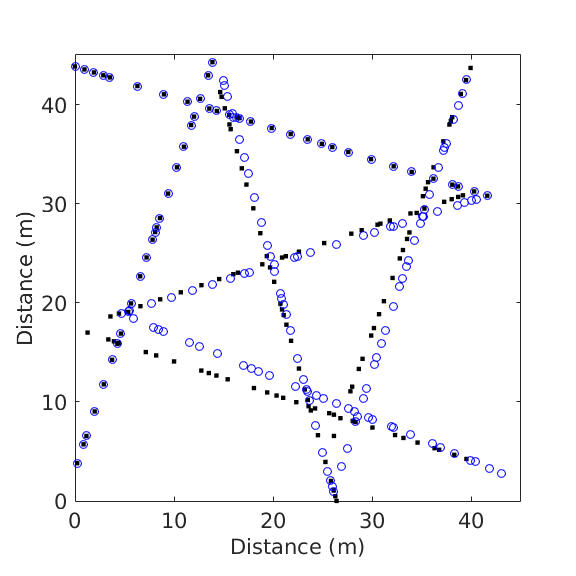
\includegraphics[width = 0.5\textwidth]{Zigzag_calOptions.png}\\
	\caption{Example of zigzag survey measurement locations calculated using difference reference vertices for each section of the zigzag. Black squares show measurement locations calculated using the original GPS coordinates of vertices (Option 1). Blue circles show measurement locations calculated using the last measurement location from the previous section as the reference vertex (Option 2). For the first and fifth vertices (located at (0, 40 m) and (0, 4 m)) the original GPS coordinates were used, which is why those sections have the same measurement locations for both options. }
	\label{fig:zigzag_location_options}
\end{wrapfigure}

Data from zigzag surveys, which include the measured snow depths and distances between adjacent measurement points, were entered to a spreadsheet. The data were then processed using the following procedure (each step corresponds with a section of the Matlab code `Import\_Zigzag.m'):
\begin{enumerate}
\item Data were imported into Matlab.
\item Categorical data, including glacier number, zigzag zone label, reference vertex, data quality, observer name, date collected, and book name, were created.
\item A structure that contained the depth data and categorical variables was created.
\item The distance of each measurement point from its reference vertex was then calculated (Figure \ref{fig:zigzag_location_options}). These locations were assumed to be a cumulative sum of distances in a straight line between two subsequent vertices. Two options exist for determining the location of the reference vertex:
 	\begin{enumerate}
	\item Option 1 calculates the distance of each point from the UTM coordinates of the reference vertex.
	\item Option 2 calculates the distance of each point from the end of the previous line of measurements. Since the cumulative distance (measured using an avalanche probe) of each zigzag section was not equivalent to the distance between UTM coordinates of each vertex (due to error in GPS and/or walking between vertices not along a straight line), this option takes the reference for each line to be the end of the previous line. The coordinates of the vertices were used for the start of each `Z' shape (ZZ01 and ZZ05).
	\end{enumerate}
\item The final processing removes poor quality data and converts snow depth to snow water equivalent (SWE) based on the density calculated from the average SWE values measured with the Federal Sampler in each zigzag (see Section \ref{sec:zigzag_density}).
\end{enumerate}

\subsection{Snow density}
\label{sec:zigzag_density}

The snowpit and Federal Sampler measurements were entered into a spreadsheet and the snow density from each measurement was calculated. For snowpit measurements the snow density was calculated by multiplying the measured density from each wedge sample by the thickness of the sample and summing these values. This is known as an integrated snow density and it encompasses the whole snow column. A density of 917 kg m$^{-3}$ was applied to ice layers and a density of 600 kg m$^{-3}$ was applied to layers that were described as `hard' and were too difficult to sample. To determine the error in estimating integrated snow density, the values of ice density, ice-layer thickness, and the `hard' layer density were varied between 700 and 917 kg m$^{-3}$, $\pm$ 1 cm (representing 20-100\% of the ice-layer thickness), and 500 and 600 kg m$^{-3}$, respectively.  A summary of density values and ranges is shown in Table \ref{tab:density_stats}.

\begin{table}[b!]
\centering
\caption{Mean and standard deviation (std) of snow density (kg m$^{-3}$)measured on study glaciers in snowpits and using a Federal Sampler. The number of sampling locations ($n$) is also given.}
\label{tab:density_stats}
\begin{tabular}{c|ccc|ccc}
\multirow{2}{*}{} & \multicolumn{3}{c}{\textbf{Snowpits}} & \multicolumn{3}{| c}{\textbf{Federal Sampler}} \\
 & Mean & Std & $n$ & Mean & Std & $n$ \\ \hline
\textbf{Glacier 4} & 348 & 13 & 3 & 327 & 32 & 7 \\
\textbf{Glacier 2} & 333 & 26 & 4 & 326 & 23 & 7 \\
\textbf{Glacier 13} & 349 & 26 & 10 & 307 & 32 & 31 \\ \hline
\textbf{All} & 342 & 26 & 10 & 316 & 31 & 31
\end{tabular}
\end{table}

Density values determined from Federal Sampler measurements that were deemed to be unrepresentative of the local snow pack, including measurements where the inner core length was less than 70\% of the snow depth or where density values were exceptionally high (e.g. 490 kg m$^{-3}$), were flagged as poor quality and removed. The remaining Federal Sampler density values were then averaged for each measurement location. The data were processed in Matlab as follows (each step corresponds with a section of the Matlab code `Import\_Density.m'): 
\begin{enumerate}
\item Data were imported into Matlab and poor quality data were removed. 
\item The mean snow density (Federal Sampler), snow density standard deviation, and number of good measurements were calculated for each zigzag survey .
\item The mean snow density (Federal Sampler), snow density standard deviation, and number of good measurements were calculated. 
\item A structure with the processed data was created (\texttt{Density}).
\end{enumerate}

The final version of the \texttt{Density} structure includes five fields:
\begin{itemize}
\item[]\texttt{Density.snowpit} contains snow density data from snowpits. Columns correspond to snowpit label, integrated density, Easting, Northing, elevation, minimum density, maximum density, snow depth.
\item[]\texttt{Density.pitANDtube} includes data from locations where measurements were taken in a snowpit and with a Federal Sampler. Columns correspond to snowpit label, Federal  Sampler mean density, standard deviation, minimum Federal Sampler-derived density, maximum Federal Sampler-derived density, number of observations, snowpit-derived density, site elevation, minimum snowpit density, and maximum snowpit density.
\item[]\texttt{Density.tube} includes Federal Sampler data. Columns correspond to location label, density mean, standard deviation, minimum and maximum, number of good quality observations, Easting, Northing, elevation, and snow depth. 
\item[]\texttt{Density.zigzagtube} includes density values at each zigzag location estimated using a Federal Sampler. Columns correspond to zigzag label, mean density, standard deviation, number of observation, and site elevation. 
\item[]\texttt{Density.SWEdepth} is a summary of all the Federal Sampler derived density data and corresponding snow depth measurements. Columns correspond to location label, mean probe depth, depth measured by the Sampler, and snow density measured using the Federal Sampler. 
\end{itemize}

\subsection{Snow water equivalent (SWE)}

The conversion of measured snow depth to snow water equivalent (SWE) could not be done at all measurement locations because snow density was not measured at all locations where snow depth was measured. This meant that the density measurements need to be interpolated. A subset of appropriate interpolation methods was chosen for this project. In the absence of a clear justification for choosing one option over the other, all options were carried forward in the analysis. A schematic of the interpolation method choices is shown in Figure \ref{fig:SWEoptions}. 

Four main interpolation methods are used \citep{McGrath2015, Elder1991}. The first assumes a uniform spatial distribution of density, calculated as the mean from all measurement locations on all three glaciers, over the entire study area. The second  also assumes a uniform spatial distribution of density but uses a mean density for individual glaciers (different value for each glacier). The third and fourth methods involve spatially variable density values. One of these methods involves using a regression of elevation and measured density values to interpolate between measurement locations. The other spatially variable interpolation method uses an inverse-distance weighted mean for interpolation. 

Since the snowpit-derived densities and Federal Sampler-derived densities had no discernible relationship, the two density datasets are kept separate. This means that for each density interpolation option, there are two outputs. In the end, there are eight different interpolations of density that are carried forward throughout the study, which allows for a range of SWE estimates to be made. 

The eight density distributions can be classified as using either snowpit-derived densities (SP) or Federal Sampler-derived densities (FS) and as using a certain method, indicated by a number.
\begin{itemize}
	\item[SP1] Calculates the mean density of all snowpit measurements.
	\item[FS1] Calculates the mean density of all Federal Sampler measurements.
	\item[SP2] Calculates the mean density for each glacier using the snowpit measurements. 
	\item[FS2] Calculates the mean density for each glacier using the Federal Sampler measurements. 
	\item[SP3] Calculates the slope and intercept of the best-fit regression line of snowpit densities with elevation for each glacier using the `fit' function and then uses slope and intercept to determine density for all elevations associated with each measurement location.
	\item[FS3] Calculates the slope and intercept of the best-fit regression line of Federal Sampler densities with elevation for each glacier using the `fit' function and then uses the slope and intercept to determine density for all elevations associated with each measurement location.
	\item[SP4] Determines the distance between each measurement location and each snowpit and then calculates the inverse-distance weight. For each measurement location, each snowpit density is then multiplied by its weight and these values are added together and divided by the sum of all weights. 
	\item[FS4] Determines the distance between each measurement location and each Federal Sampler and then calculates the inverse-distance weight. For each measurement location, each Federal Sampler density is then multiplied by its weight and these values are added together and divided by the sum of all weights. 
	\end{itemize}


{
\begin{wrapfigure}{r}{\textwidth} 
	\centering
	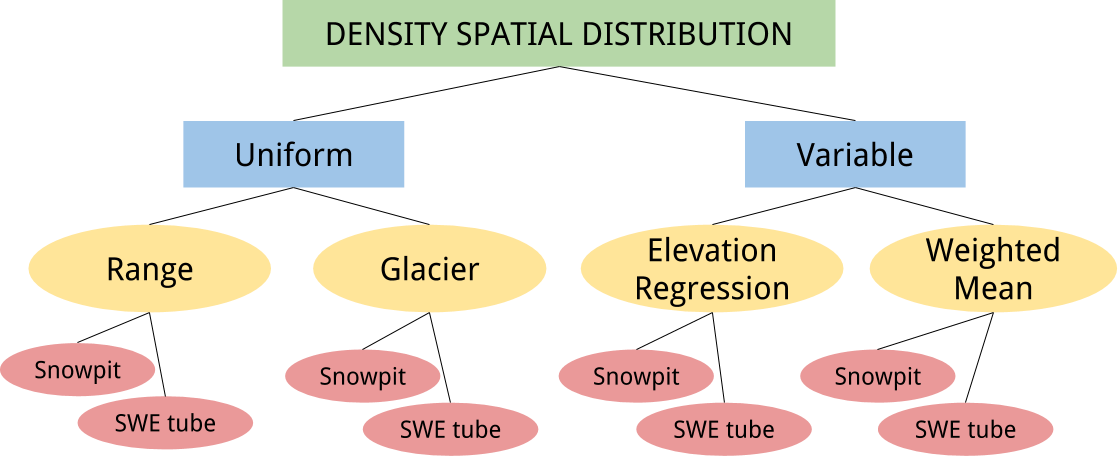
\includegraphics[width = \textwidth]{SWEoptions.png}\\
	\caption{Relationship between various ways to interpolate between density measurements for the calculation of SWE.}
	\label{fig:SWEoptions}
\end{wrapfigure}
}

The final SWE values for each measurement location are calculated in Matlab using the following steps (this corresponds to the script `Import\_SWE.m'):
\begin{enumerate}
\item Snow depth values from transects, zigzags, and extra measurements is complied into a single structure called `SWE'.
\item The elevation of each measurement location according to the SPOT5 DEM was found in QGIS and the elevations are imported to Matlab and assigned to their respective depth measurement values.
\item The density values for each snow depth measurement location were estimated according to the chosen method. SWE was then calculated. 
\end{enumerate}
To select the desired density calculation option (or to cycle through all options), change the value of \texttt{options.DensitySWE} to the appropriate option number.

The final version the \texttt{SWE} structure includes three rows that correspond to Glacier 4, 2, and 13 and ten fields. The fields are: 
\begin{itemize}
\item \texttt{book} (field book where measurement is written)
\item \texttt{comments} (any comments noted by observer)
\item \texttt{density} (the density value used to calculate SWE)
\item \texttt{depth} (mean depth measured at each sampling location, $n=3$ usually)
\item \texttt{glacier} (glacier number where measurement was taken)
\item \texttt{label} (measurement point reference label; for transects this is the waypoint number and relative position, for other measurements this is a label associated with transect and location)
\item \texttt{pattern} (transect, or set of transects, that include the measurement)
\item \texttt{person} (initials of observer)
\item \texttt{swe} (estimated SWE value)
\item \texttt{utm} (the Easting and Northing for the measurement location as well as the DEM elevation). 
\end{itemize}
For example, to access the SWE values for Glacier 2, one would type \texttt{SWE(2).swe}. 

The \texttt{SWE} structure includes all data that is collected for each glacier. If there is a need to remove the zigzag data or keep only the zigzag data, the script `ZigzagRemoval.m' can be run. Set the option for including or excluding zigzag data in the script `OPTIONS.m'.




\bibliography{/home/glaciology1/Documents/MastersDocuments/MastersLit}
\bibliographystyle{igs}

\end{document}